% En esta sección considere solo lo que se va a comprometer durante el curso. Considere el calendario escolar como límite de tiempo.
%--------------------------------------------------------------------
\section{Descripción metodológica}
Para el desarrollo del sistema emplearemos una metodología de desarrollo ágil llamada Programación extrema, la cual consiste en realizar entregas cortas al cliente por pequeños lapsos de tiempo, se adapta a pequeños equipos y puede lograr un sistema de calidad en poco tiempo.



\section{Desglose de actividades}

La metodología de desarrollo estará compuesta de 4 principales actividades:
\\\\
\textbf{Planeación}. Una vez identificados los requerimientos descritos por el cliente(historias de usuario) se le asignará una prioridad a cada requerimiento ya sea Alta o Baja, posteriormente se estimará el tiempo para cumplir dicho requerimiento.
\\\\
\textbf{Diseño}. Las historias de usuario serán trasladados a tarjetas CRC(Clase-Responsabilidad-Colaborador) esto con la finalidad de identificar y organizar las clases orientadas a objetos con más facilidad.
\\\\
\textbf{Codificación}. Primero las historias de usuario se programaran de manera individual haciendo pruebas unitarias antes de integrarse al sistema principal esto con la razón de que el desarrollador esté más seguro y conozca con exactitud lo que se tiene que hacer. Posterior a esto se llevará a cabo la programación en pares para que así haya mayor retroalimentación y uno compruebe el trabajo de otro. Al finalizar se hará el proceso de refactorización, esto con el fin de hacer más legible y mejorar el código fuente.
\\\\
\textbf{Pruebas}. Como ya se había mencionado anteriormente se deben llevar a cabo pruebas unitarias antes de la codificación. También se deben realizar pruebas de aceptación, esta consiste en entregar un avance del sistema al cliente con las nuevas historias de usuario  ya integradas.
\\\\
Estas 4 actividades se irán repitiendo constantemente hasta la entrega final del proyecto.

\section{Cronograma de actividades}
El plan de trabajo consiste en 5 iteraciones, cada una con sus correspondientes actividades mencionadas anteriormente con la diferencia en que la estapa de Pruebas se divide en 2, pruebas unitarias del sistema y pruebas de aceptación que implica la entrega y revisión al cliente. Como se puede observar en cronograma sólo se trabajarán 5 días a la semana (de lunes  a viernes), por día se trabajaran 4 hrs. El plan contempla 12 semanas y 4 entregas parciales antes de la entrega final.
\begin{figure}[h!]
	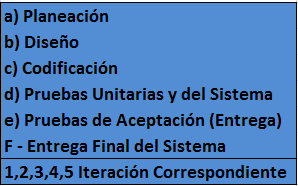
\includegraphics[width=6.5cm, height=4.5cm]{xp1.png}
	
\end{figure}
\begin{figure}[h!]
	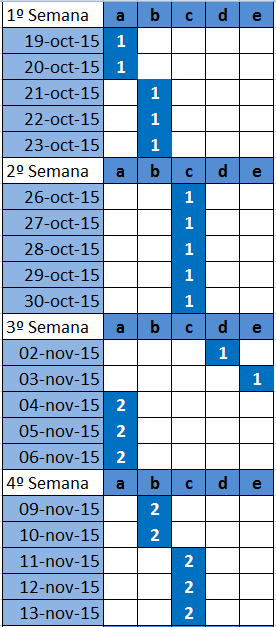
\includegraphics[width=5.5cm, height=13cm]{xp2.PNG}
	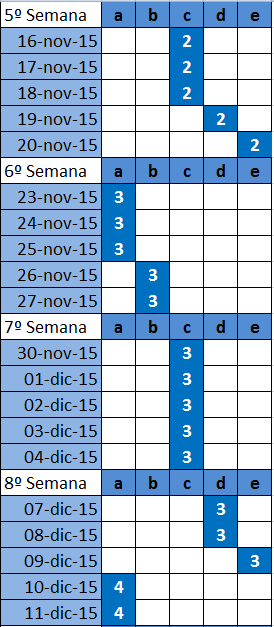
\includegraphics[width=5.5cm, height=13cm]{xp3.PNG}
	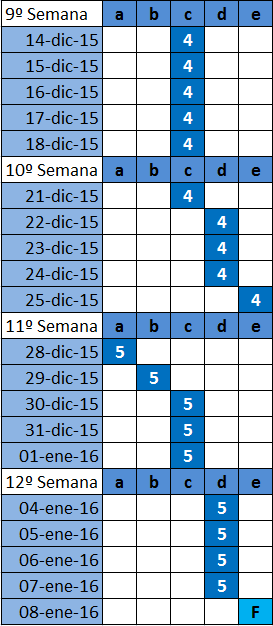
\includegraphics[width=5.5cm, height=13cm]{xp4.PNG}
\end{figure}
\begin{itemize}
	\item \textbf{ETAPA 1}: Para la primera etapa se llevarán a cabo los siguientes requerimientos: RF1, RF3, RF5 y RF19 ya que abarca en su mayoría la creación de la Base de Datos, Modelado y Scripts.
	\item \textbf{ETAPA 2}: Para la segunda etapa se llevarán a cabo los siguientes requerimientos: RF10, RF13, RF16 y RF20 los cuales definen el registro de toda la información, para ello se realizarán las distintas pantallas con sus correspondientes formularios.
	También en esta etapa se llevarán a cabo los siguientes requerimientos: RF2, RF4 y RF6  los cuales definen las pantallas donde se muestra toda la información.
	\item \textbf{ETAPA 3} Para la tercera etapa se llevarán a cabo los siguientes requerimientos: RF12, RF15 y RF18 los cuales se refieren al proceso de eliminar registros.
	También en esta etapa se llevarán a cabo los siguientes requerimientos: RF11, RF14 y RF17  los cuales definen la modificación de registros.
	\item \textbf{ETAPA 4}: Para la cuarta etapa se llevarán a cabo los siguientes requerimientos: RF21, RF22 y RF23 los cuales se refieren a la administración de usuarios.
	También en esta etapa se llevarán a cabo los siguientes requerimientos: RF7, RF8 y RF9  los cuales se refiere a la generación de informes personalizados.
	\item \textbf{ETAPA 5}: En esta última etapa se llevarán a cabo requerimientos que vayan surgiendo a lo largo de los próximos 2 meses que no se hayan considerado en los primeros análisis, también esta etapa servirá para detectar errores y realizar pruebas de todo el sistema.
	
\end{itemize}
\section{Equipo de trabajo}
\begin{itemize}
	\item \textbf{Lider de Proyecto y Desarollador}
	\\\\
	\textbf{Ivan Baltazar:} 
	\\ Sus responsabilidades son dirigir al equipo y asignar equitativamente las tareas, servir de apoyo para los integrantes y generar un buen ambiente de trabajo.
	\item\textbf{ Analista, Diseñador y Desarrollador}
	\\\\
	\textbf{{Daniel López -}}
	\textbf{Arturo Escutia -} 
	\textbf{Miguel Angel Medina:} 
	\\ \\ Debe cumplir con las tareas que se le asignan de manera eficiente, ser responsable, respetuoso con los demás integrantes y aplicar correctamente sus conocimientos en desarrollo de sistemas. Tener amplio conocimieno en el área de desarrollo y contar con experiencia. Debe saber comunicarse con el lider de proyecto para hacerle saber la situación del equipo.
\end{itemize}	

\section{Entregables}
\begin{itemize}
	\item Código fuente de todo el sistema.
	\item Base de datos (Modelo Entidad-Relación y Scripts).
	\item CRC’s
	\item Casos de uso
	\item Diagramas de clase
	\item Diagramas de secuencia
	\item Pantallas
\end{itemize}
\section{Resumen de tiempo y costo}
El equipo esta compuesto por 4 integrantes los cuales trabajarán 4 horas al día esto durante 12 semanas, de lunes a viernes lo que da un total de 60 días y 240 horas por integrante. 
\\\\
Tomando en cuenta los factores anteriores y que cada trabajador llevará a cabo todo tipo de actividades (Planeación,Diseño,Desarrollo y Pruebas) se cobrará un total de 120 pesos la hora por trabajador lo cual da un total de 28,800 pesos que al multiplicar por los 4 integrantes del equipo sumarian 115,200 pesos eso sólo considerando el recurso humano, más aparte la renta de servidor el cual se sugiere pagar el primer año completo aunque cabe mencionar que esos ya serían gastos aparte como el mantenimiento y la capacitación del personal para el uso del sistema.
